% !TeX spellcheck = es_MX-SpanishMexico
%----------------------------------------------------------------------------------------------------
%                           		  ENTRE LÍNEAS DE TIERRA

% Curso: Arqueología Bíblica
% Módulo 1: Introducción, Definiciones y Conceptos
% Elabora: Rodrigo Gerardo Trejo Arriaga

%----------------------------------------------------------------------------------------------------

% FORMATO DEL DOCUMENTO


\documentclass[11pt]{article} % Letra estandar

\usepackage[utf8]{inputenc}

%\usepackage{tgadventor}
%\renewcommand{\familydefault}{\sfdefault}

\usepackage[light,math]{iwona}

\usepackage[T1]{fontenc}


\usepackage[spanish]{babel}
\addto\captionsspanish{\renewcommand{\abstractname}{\large{Introducción}}}

\usepackage[margin=1in,letterpaper]{geometry}

\usepackage{fancyhdr} % Paquete para personalizar encabezado y pie de página
\pagestyle{fancy} % Establece que personalizaremos el pie de pagina y el encabezado
\setlength{\headheight}{13.59999pt} % Establece la altura del encabezado
\fancyhead[R]{\textcolor{darkBlue}{Teoría de la Computación}} % Encabezado derecho
\fancyhead[L]{\textit{\textcolor{darkBlue}{Escuela Superior de Cómputo}}} % Encabezado izquierdo
\fancyfoot[L]{\textit{\textcolor{darkBlue}{Práctica 2}}} % Pie de página izquierdo 
\fancyfoot[R]{\textcolor{darkBlue}{\thepage}} % Pie de página  derecho
\fancyfoot[C]{} % Elimina la nueración central de páginas en el pie de página
\renewcommand{\headrulewidth}{0.5pt} % Grosor de la linea de encabezado
\renewcommand{\footrulewidth}{0.5pt} % Grosor de la linea de pie de página

\usepackage{enumitem}

\usepackage{changepage}

\usepackage{graphicx}

\usepackage{tabularx}

\setlength{\parskip}{8pt}

\usepackage{xcolor}
\definecolor{darkBlue}{rgb}{0,0,0.31}
%\definecolor{darkBlue}{rgb}{0,0,0.5}
\definecolor{munsell}{rgb}{0.0, 0.5, 0.69}
\definecolor{indigo}{rgb}{0.0, 0.25, 0.42}
\renewcommand{\footrulewidth}{2pt}
\renewcommand{\footrule}{\hbox to\headwidth{\color{darkBlue}\leaders\hrule height \footrulewidth\hfill}}

\usepackage{colortbl}

\usepackage{titlesec}
\titleformat{\section}
{\normalfont\Large\bfseries\color{darkBlue}}{\thesection.}{1em}{}

\usepackage{tabularx}

\usepackage{textcomp}

\usepackage{titling}

\usepackage{apacite}
\bibliographystyle{apacite}

%\usepackage{natbib}
%\setlength{\bibsep}{6pt}

\usepackage{setspace}

\usepackage{listings}


\lstset{
	language=Python,                % Lenguaje del código (Python en este caso)
	basicstyle=\ttfamily,           % Estilo de fuente
	keywordstyle=\color{blue},      % Estilo para las palabras clave
	commentstyle=\color{green},     % Estilo para los comentarios
	numbers=left,                   % Colocar números de línea a la izquierda
	numberstyle=\tiny\color{gray},  % Estilo para los números de línea
	stepnumber=1,                   % Número de línea cada 1 línea
	tabsize=4,                      % Tamaño de la tabulación
	frame=single,                   % Colocar un marco alrededor del código
	breaklines=true,                % Romper líneas largas automáticamente
	showstringspaces=false,         % No mostrar espacios en cadenas
	escapeinside={(*@}{@*)},        % Para incluir caracteres especiales en el código
	extendedchars=true               % Permitir caracteres especiales, como acentos
}


\renewcommand{\thesection}{\Roman{section}}

%----------------------------------------------------------------------------------------------------
% CUERPO DEL DOCUMENTO

\begin{document}
	
	\begin{titlepage}
		\centering
		{
\includegraphics[width=0.25\textwidth]{descarga}\par}
		\vspace{0.5cm}
		{\bfseries\huge Escuela Superior de Cómputo \par}
		\vspace{0.7cm}
		{\scshape\LARGE Teoría de la Computación \par}
		\vspace{0.3cm}
		\vspace{3.1cm}
		{\scshape \Huge \textbf{Práctica 2:}  \par}
		\vspace{0.03cm}
		{{\LARGE \textit{Primos}} \par}
		%\vfill
		\vspace{3.5cm}
		{\Large Autor: \par}
		{\Large Rodrigo Gerardo Trejo Arriaga \par}
		%\vfill
		\vspace{3cm}
		{\Large Octubre 2023 \par}
	\end{titlepage}
	
	\begin{center}
		\vspace*{0.1cm}
		{\huge \textcolor{darkBlue}{\textbf{Práctica 2:}} \par}
		
		{\Large \textcolor{darkBlue}{\textbf{\textit{Primos}}}}
	\end{center}
	
	En la teoría de la computación, un alfabeto se define como un conjunto finito de símbolos o caracteres. Estos símbolos son la base fundamental para construir cadenas o secuencias de símbolos. Por ejemplo, en el contexto de la teoría de la computación, es común utilizar el alfabeto ${0, 1}$ para representar símbolos binarios.
	
	Una cadena, también conocida como palabra, es una secuencia finita de símbolos tomados de un alfabeto dado. Estas cadenas desempeñan un papel esencial en la representación de datos y forman la base de los lenguajes formales en la teoría de la computación.
	
	El conjunto universo, por otro lado, hace referencia a un conjunto que contiene todos los objetos posibles que son relevantes para un problema o lenguaje específico. Por ejemplo, si se trata de un lenguaje de programación, el conjunto universo podría consistir en todos los programas concebibles que se pueden escribir en ese lenguaje.
	
	En el contexto de la teoría de la computación, un lenguaje formal se define como un conjunto de cadenas (palabras) construidas a partir de un alfabeto dado. Estos lenguajes formales se utilizan para describir propiedades de las cadenas y son fundamentales en la definición de gramáticas formales, autómatas y en la resolución de diversos problemas relacionados con la informática teórica.
	
	En esta práctica presentaremos un programa que conjunta todos estos conceptos.
	
	\section{Descripción del problema}

	Este programa calcula el lenguaje binario definido por números primos. El valor de "n" puede ser introducido por el usuario o determinado automáticamente por el programa, y está restringido al rango [2, $10^7$]. El valor de "n" determina hasta qué número se calcularán y cuántos números primos existen en ese intervalo.	

	\begin{enumerate}
		\item Ejecute el programa y especifique el valor de "n" que desea utilizar para el cálculo.
		\item El programa preguntará si desea calcular otro valor de "n" o salir.
		\item Los resultados se guardarán en dos archivos de texto: uno en notación binaria y otro en notación decimal.
		\item A continuación, graficaremos el número de unos en cada cadena. El eje "x" representa las cadenas y el eje "y" representa el número de unos en cada cadena.
		\item En el informe, se explicará, calculará y graficará el caso específico cuando "n=$200^3$".
		\item Además, se calculará una segunda gráfica utilizando el logaritmo en base 10 del número de unos.
	\end{enumerate}
	
	
	\section{Resultados}
	\begin{figure}[H]
		\centering
		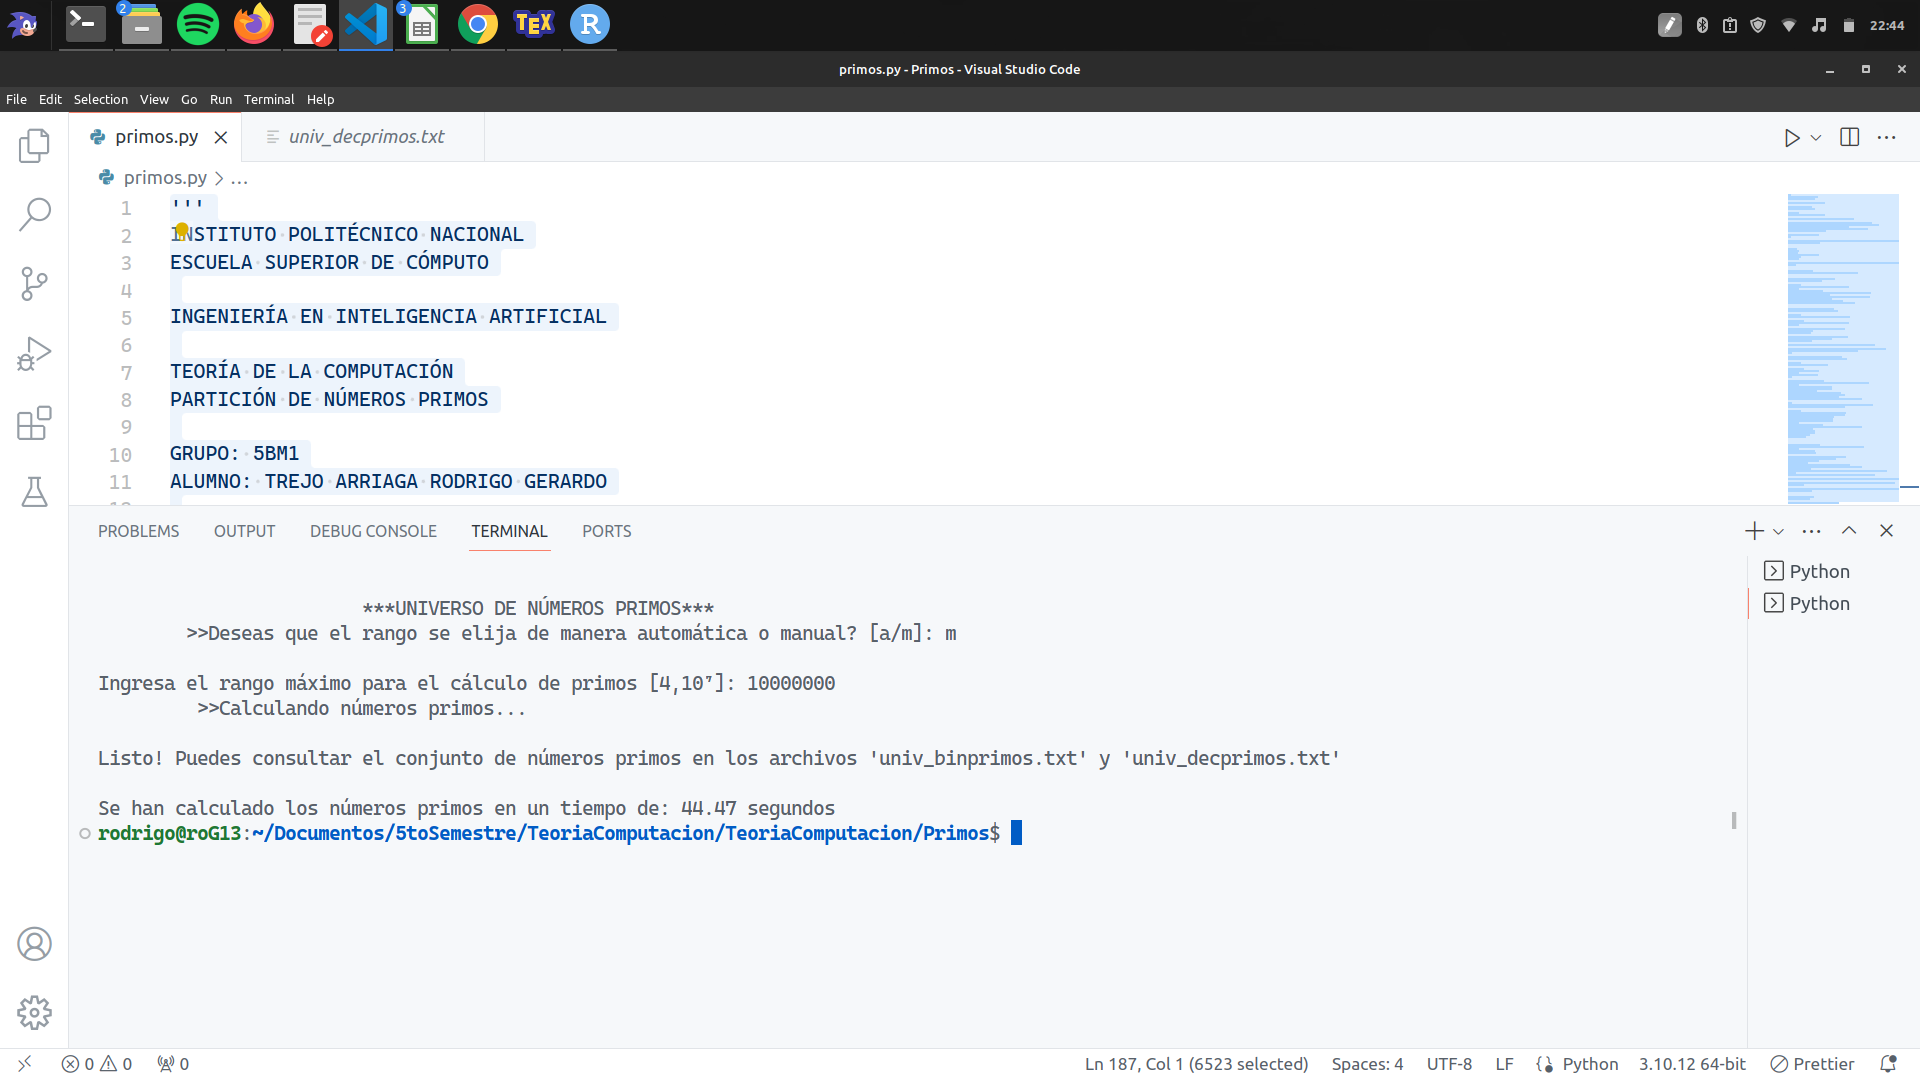
\includegraphics[width=0.8\textwidth]{imagen1.png}
		\caption{Descripción de la imagen}

	\end{figure}
	
	\begin{figure}[H]
		\centering
		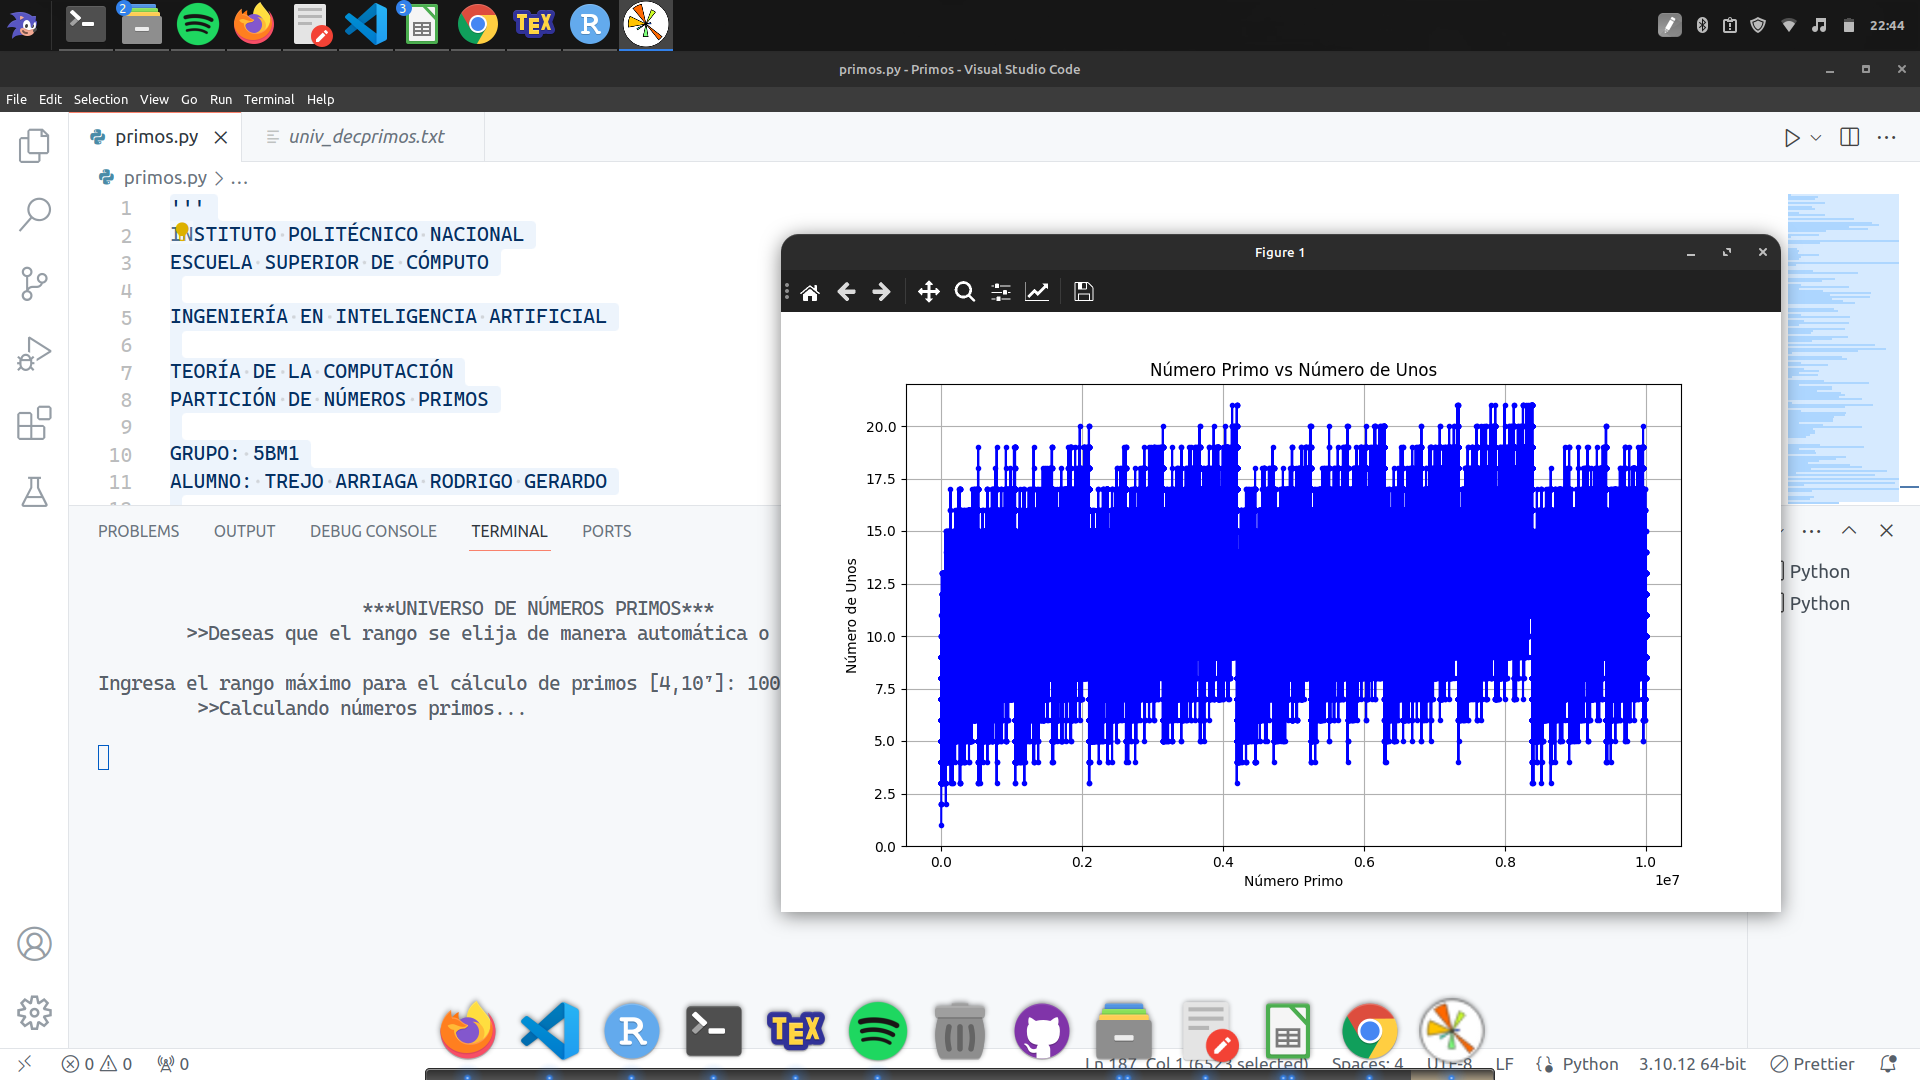
\includegraphics[width=0.8\textwidth]{imagen2.png}
		\caption{Programa terminado}
	\end{figure}
	
	\begin{figure}[H]
		\centering
		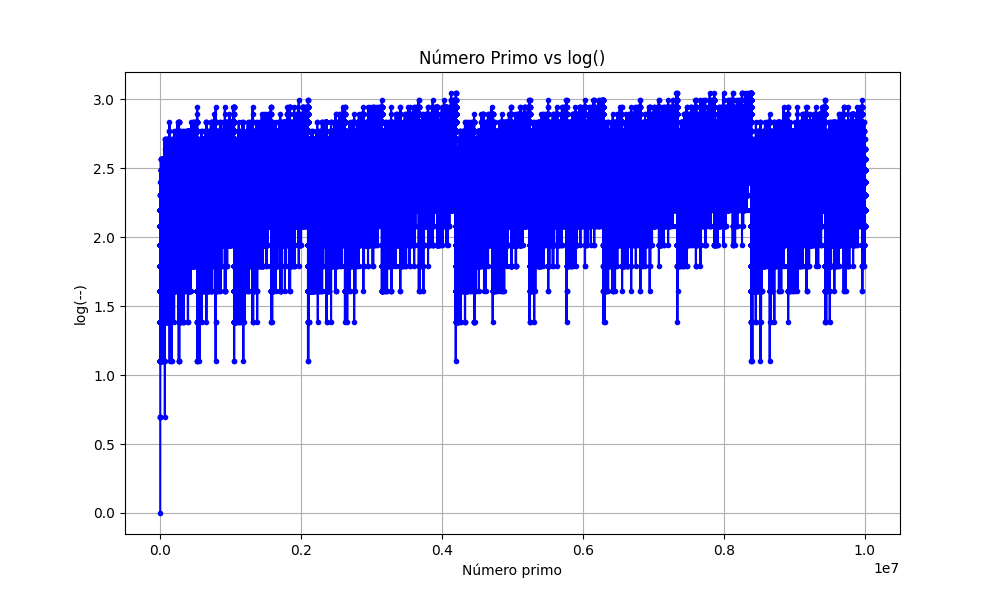
\includegraphics[width=0.8\textwidth]{imagen3.png}
		\caption{Ejecución con gráfica}
	\end{figure}
	
	\begin{figure}[H]
		\centering
		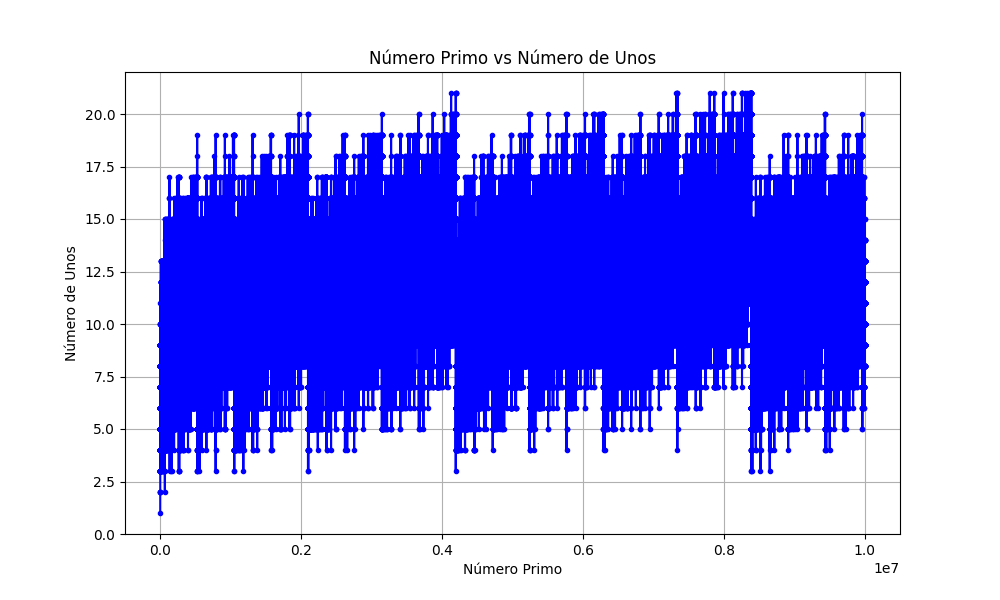
\includegraphics[width=0.8\textwidth]{imagen4.png}
		\caption{Gráfica Logaritmo}
	\end{figure}
	
	
	\section{Código de Implementación}
	
	\begin{lstlisting}
	'''
	INSTITUTO POLITÉCNICO NACIONAL
	ESCUELA SUPERIOR DE CÓMPUTO
	
	INGENIERÍA EN INTELIGENCIA ARTIFICIAL
	
	TEORÍA DE LA COMPUTACIÓN
	PARTICIÓN DE NÚMEROS PRIMOS
	
	GRUPO: 5BM1
	ALUMNO: TREJO ARRIAGA RODRIGO GERARDO
	
	ESTE PROGRAMA CREA UNA PARTICIÓN DEL UNIVERSO DE NÚMEROS PRIMOS Y:
	
	i) ALMACENA TODOS LOS NUMEROS QUE PRIMOS EN UN RANGO (TANTO EN BINARIO COMO DECIMAL)
	ii) GENERA UNA TABLA CON TODOS LOS NÚMEROS PRIMOS BINARIOS Y LOS NÚMEROS DE UNOS QUE TIENEN
	ii) GENERA UNA GRÁFICA DEL NÚMERO PRIMO VS SU NÚMERO DE UNOS 
	iii) GENERA UNA GRÁFICA DE LOS NÚMEROS PRIMOS VS EL LOGARITMO DEL NÚMERO DE UNOS
	PARA APRECIAR MEJOR SU CRECIMIENTO
	
	ÚLTIMA MODIFICACIÓN: 13/10/2023
	'''
	
	#  --------------------------------------------------------------------------------------------------------------------
	# MÓDULOS Y LIBRERÍAS IMPORTADAS
	
	
	import os
	import time
	import csv
	import matplotlib.pyplot as plt
	import random
	import math
	
	#  --------------------------------------------------------------------------------------------------------------------
	# CLASES
	
	
	class ParticionNumPrimos:
	"""Clase que genera la partición del universo de números primos"""
	
	
	def __init__(self, fin_rango: int) -> None:
	"""Constructor de la clase
	
	Args:
	fin_rango (int): Límite del rango de la partición
	"""
	self.fin_rango = fin_rango 
	self.arch_binprimos =  open(f"univ_binprimos.txt", "w+", encoding="utf-8") 
	self.arch_binprimos.write("Σ = {")
		self.arch_decprimos =  open(f"univ_decprimos.txt", "w+", encoding="utf-8")
		self.arch_decprimos.write("Σ = {")  
			self.arch_tablasUnos = open(f"tabla.csv", "w+")
			self.arch_tablasUnos.write("Numero, Cantidad de Unos\n" )  
			
			
			def es_primo(self, num_test: int) -> bool:
			"""Método que indica si un número es primo
			
			Args:
			num_test (int): Número que se verifica si es primo
			
			Returns:
			bool: Bandera que dice si el número es primo o no
			"""
			
			# Comprobamos si n es igual a 2 (único primo par)
			if num_test == 2:
			return True
			
			# Comprobamos si n es menor que 2 o es un número par
			if num_test < 2 or not num_test % 2:
			return False
			
			sqrt_n = int(num_test**0.5) + 1  # Calculamos la raíz cuadrada de n + 1 una vez
			
			# Comprobamos si n es divisible por cualquier entero impar entre 3 y la raíz cuadrada de n
			return not any(num_test % i == 0 for i in range(3, sqrt_n, 2))
			
			
			def convertir_a_binario(self, numero: int) -> str:
			"""Método que convierte un número decimal a binario
			
			Args:
			numero (int): Número decimal
			
			Returns:
			str: Número binario
			"""
			return bin(numero)[2:]
			
			
			def calcular_rango_primos(self):
			"""Método que escribe en archivos los números primos decimales y binarios
			"""
			for i in range(2, self.fin_rango+1):
			bandera_primo = self.es_primo(i)
			if bandera_primo:
			binario = self.convertir_a_binario(i)
			self.arch_binprimos.write(f"{binario}, ")
			self.arch_decprimos.write(f"{i}, ")
			self.arch_tablasUnos.write(f"{i}, {binario.count('1')}\n")
			
			
			def plotear_grafico(self, x: list, y:list, titulo:str, label_x:str, label_y:str):
			"""Método que plotea una gráfica según dos listas
			
			Args:
			x (list): Lista de datos que irán en el eje x 
			y (list): Lista de datos que irán en el eje y
			titulo (str): Título de la gráfica
			label_x (str): Etiqueta del eje x
			label_y (str): Etiqueta del eje y
			"""
			plt.figure(figsize=(10, 6))
			plt.plot(x, y, marker='o', linestyle='-', color='b', markersize=3)
			plt.title(titulo)
			plt.xlabel(label_x)
			plt.ylabel(label_y)
			plt.grid(True)
			plt.show()
			
			
			
			def graficar_num_unos(self):
			"""Método que obtiene la gráfica del número de unos por número primo
			"""
			numeros_primos = []
			numeros_de_unos = []
			
			with open("tabla.csv", newline='') as archivo_csv:
			reader = csv.DictReader(archivo_csv)
			for fila in reader:
			try:
			numeros_primos.append(int(fila["Numero"]))
			numeros_de_unos.append(int(fila[" Cantidad de Unos"]))
			except:
			print(f"numero = {fila['Numero']} Cantidad = {int(fila[' Cantidad de Unos'])}")
			
			logaritmo = [0 if valor == 0 else math.log(valor) for valor in numeros_de_unos]
			
			self.plotear_grafico(numeros_primos, numeros_de_unos, 'Número Primo vs Número de Unos', 'Número Primo', 'Número de Unos', )
			
			self.plotear_grafico(numeros_primos, logaritmo, 'Número Primo vs log()', 'Número primo', 'log(--)')
			
			
			#  --------------------------------------------------------------------------------------------------------------------
			# FUNCIÓN PRINCIPAL MAIN
			
			
			if __name__ == "__main__":
			os.system('clear')
			
			print("\t\t\t***UNIVERSO DE NÚMEROS PRIMOS***")
			modo = input("\t>>Deseas que el rango se elija de manera automática o manual? [a/m]: ")
			while modo.lower() != "a" and modo.lower() != "m":
			print("Modo inválido, ingreséselo nuevamente para continuar")
			modo = input("\t>>Deseas que 'n' se elija de manera automática o manual? [a/m]: ")
			
			match modo:
			case "m":
			n = int(input("\nIngresa el rango máximo para el cálculo de primos [4,10⁷]: "))
			while n > 10000000 and n < 4:
			print("Rango incorrecto! Inténtalo nuevamente.")
			n = int(input("\nIngresa el rango máximo para el cálculo de primos [4,10⁷]: "))
			case _:
			n = random.randint(0, 10000000)
			print(f"\nSe ha elegido un n={n}")
			
			print("\t >>Calculando números primos...\n")
			inicio = time.perf_counter()
			t = ParticionNumPrimos(n)
			t.calcular_rango_primos()
			fin = time.perf_counter()
			t.arch_binprimos.write("}")
		t.arch_binprimos.close()
		t.arch_decprimos.write("}")
	t.arch_decprimos.close()
	t.arch_tablasUnos.close()
	t.graficar_num_unos()
	tiempo_transcurrido = fin - inicio
	
	print("Listo! Puedes consultar el conjunto de números primos en los archivos 'univ_binprimos.txt' y 'univ_decprimos.txt'")
	
	print(f"\nSe han calculado los números primos en un tiempo de: {tiempo_transcurrido:.2f} segundos")
	
	\end{lstlisting}
	
	
	
	
	
\end{document}